% EDA report for the Speed Dating data. Build from this folder (eda/report/), with Neo4j running:
%   python figures.py
%   pdflatex eda_report.tex
\documentclass[10pt,a4paper]{article}
\usepackage[T1]{fontenc}
\usepackage{lmodern}
\usepackage{microtype}
\usepackage[a4paper,margin=1.7cm,top=1.5cm,bottom=1.6cm]{geometry}
\usepackage{graphicx}
\usepackage{booktabs}
\usepackage[font=small,labelfont=bf,skip=3pt]{caption}
\usepackage{subcaption}
\usepackage[hidelinks]{hyperref}

\graphicspath{{figures/}}
\setlength{\parskip}{3pt}
\setlength{\parindent}{0pt}
\setlength{\textfloatsep}{8pt}
\setlength{\floatsep}{6pt}
\setlength{\intextsep}{6pt}
\makeatletter
\renewcommand\section{\@startsection{section}{1}{\z@}{-1.2ex plus -.5ex}{0.5ex}{\normalfont\large\bfseries}}
\renewcommand\subsection{\@startsection{subsection}{2}{\z@}{-1ex plus -.3ex}{0.3ex}{\normalfont\normalsize\bfseries}}
\makeatother
\newcommand{\compactlist}{\setlength{\itemsep}{0pt}\setlength{\parskip}{0pt}\setlength{\topsep}{2pt}}

\begin{document}

\begin{center}
  {\Large\bfseries Speed Dating Data: Exploratory Data Analysis}\\[2pt]
  {\small Kacper Kuźnik \quad·\quad Aleksander Hanski \quad·\quad Piotr Masłowski}
\end{center}
\vspace{-4pt}

\section{Data}

The data come from a speed-dating experiment run at Columbia Business School in 2002--2004
(\href{https://www.kaggle.com/datasets/annavictoria/speed-dating-experiment/data}{Kaggle}).
Participants, mostly graduate students, filled in a sign-up survey and attended one of 21 events
(\emph{waves}, 9--44 people each). At an event everyone had a four-minute date with every participant of the
opposite sex and then said \emph{yes} or \emph{no}; a \textbf{match} means both said yes. We model this
as a graph: people are nodes, dates are edges, and the task is to predict which edges are matches.

\begin{table}[h]
\centering\small
\begin{tabular}{@{}lrlr@{}}
\toprule
people (nodes) & 544 \;(269 women, 275 men) & dates per person & 4--22 (median 16) \\
dates (edges)  & 4,105 & matches per person & 0--14 (median 2) \\
matches        & 675 \;(16.4\% of dates) & match rate per event & 8\%--31\% \\
\bottomrule
\end{tabular}
\caption{The graph after preprocessing.}
\end{table}
\vspace{-6pt}

\section{Preprocessing}

The raw file (8,378 rows $\times$ 195 columns) has one row per person per date, and its column names are
codes that must be looked up in the codebook (e.g.\ \texttt{attr1\_1} = how much a person values
\emph{attractive} at sign-up). We keep only the 40 sign-up survey columns, since anything recorded during
or after a date would leak the outcome, and build one profile per person and one row per date. Small
fixes: hobby scores are clipped to 0--10, the six ``what do you look for'' answers (a 100-point split)
are turned into shares that add up to 1, and codes become labels. Seven people who skipped practically
the whole survey (34--37 of 37 answers missing) are dropped with their 79 dates, as the model would see
them only as imputed medians. In the remaining profiles 536 of 544 people answered everything; the other
8 miss 1--5 answers, which training fills with the median.

\section{Exploratory analysis}

\subsection{The graph and the participants}

People only dated others at their own event, so the graph splits into 21 disconnected clusters
(Fig.~\ref{fig:graph}a). Within an event the dates form a complete bipartite graph: everyone met everyone of
the opposite sex (Fig.~\ref{fig:graph}b). Matches are sparse: the median person has 2, and 102 people (19\%)
have none. The match rate also varies a lot between events, from 8\% to 31\%.

\begin{figure}[h]
\centering
\begin{subfigure}[t]{0.49\textwidth}\centering
  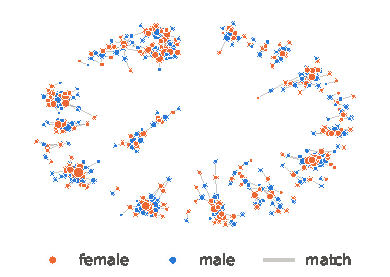
\includegraphics[width=\linewidth]{network}
  \caption{Match network. Each cluster is one event; node size = number of matches.
  The 102 people without a match are not shown.}
\end{subfigure}\hfill
\begin{subfigure}[t]{0.49\textwidth}\centering
  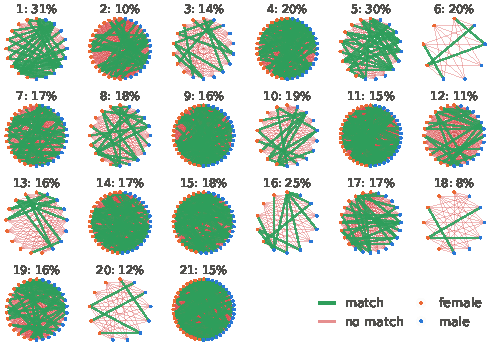
\includegraphics[width=\linewidth]{events}
  \caption{Every date, one circle per event (label: event and its match rate). Women on the left half,
  men on the right; each line is one date.}
\end{subfigure}
\caption{The match graph and all dates per event.}
\label{fig:graph}
\end{figure}

Most participants are 21--30 (88\%; median age 26 for women, 27 for men; Fig.~\ref{fig:people}a). Both
genders came mainly for a fun night out (about 42\%) or to meet new people (32--37\%); only 5\% of women and
10\% of men came ``to get a date'', and 3--5\% for a serious relationship. Fields of study differ strongly:
36\% of men study business/economics and 16\% engineering, while women are spread evenly over social science,
education, natural sciences, business and social work (11--13\% each).

\begin{figure}[h]
\centering
\begin{subfigure}[t]{0.49\textwidth}\centering
  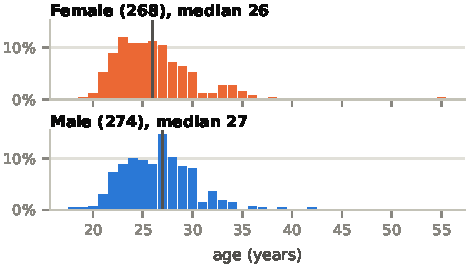
\includegraphics[width=\linewidth]{age}
  \caption{Age, as the share of each gender per year.}
\end{subfigure}\hfill
\begin{subfigure}[t]{0.49\textwidth}\centering
  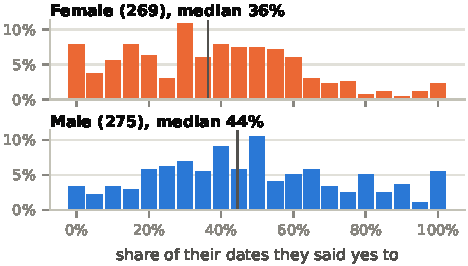
\includegraphics[width=\linewidth]{picky}
  \caption{Share of their dates each person said yes to.}
\end{subfigure}
\caption{Age of the participants and how selective they were.}
\label{fig:people}
\end{figure}

\begin{figure}[h]
\centering
\begin{subfigure}[t]{0.49\textwidth}\centering
  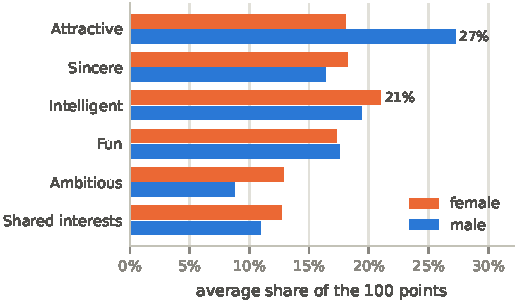
\includegraphics[width=\linewidth]{looking_for}
  \caption{\emph{Stated}: average share of points given to each attribute at sign-up.}
\end{subfigure}\hfill
\begin{subfigure}[t]{0.49\textwidth}\centering
  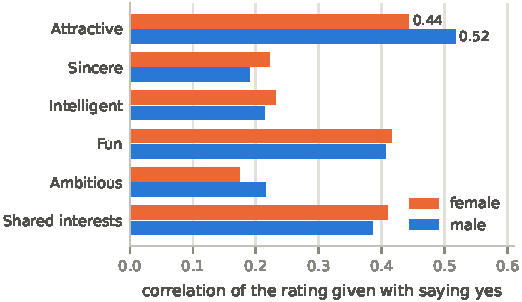
\includegraphics[width=\linewidth]{drives_yes}
  \caption{\emph{Revealed}: correlation between the rating given to a partner and saying yes.}
\end{subfigure}
\caption{What people say they look for vs what goes with a yes.}
\label{fig:prefs}
\end{figure}

\subsection{Stated vs revealed preferences}

Asked at sign-up, men put attractiveness far ahead (27\% of their points), while women spread their points
more evenly with intelligence first (21\%) and value ambition and shared interests more than men
(Fig.~\ref{fig:prefs}a). Both sexes overestimate how much the other side cares about looks: women think men
give 36\% to attractiveness, men think women give 25\% (vs 27\% and 18\% actually stated). Decisions tell a
different story (Fig.~\ref{fig:prefs}b): for \emph{both} genders the rating of attractiveness is the
attribute most associated with a yes (women 0.44, men 0.52), followed by fun and shared interests (about
0.4), while intelligence and sincerity, which women rank first when asked, matter much less (about 0.2).

\begin{figure}[h]
\centering
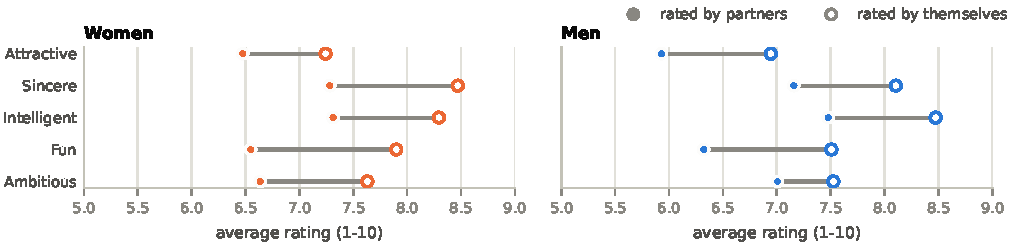
\includegraphics[width=\textwidth]{self_vs_partners}
\caption{Self-rating at sign-up (hollow) vs the average rating received from date partners (filled), 1--10.}
\label{fig:self}
\end{figure}

\subsection{Self-image and pickiness}

Everyone rates themselves higher than their partners did, on every attribute and mostly by about one point
(Fig.~\ref{fig:self}). The largest gap is for \emph{fun} (women 7.9 vs 6.5, men 7.5 vs 6.3), and men rate
their own looks a full point above what their dates gave them (7.0 vs 5.9). Men are also less selective
(Fig.~\ref{fig:people}b): the median man said yes to 44\% of his dates, the median woman to 36\%. Both
distributions are wide; 21 women and 9 men said yes to nobody, 6 women and 15 men to everyone.

\section{Implications for the model}

\begin{itemize}\compactlist
  \item \textbf{Class imbalance.} Only 16.4\% of dates are matches.
  \item \textbf{Graph structure.} Events are disconnected and many people have 0--2 matches.
\end{itemize}
These are possibly some obstacles, but we will overcome them!

\end{document}
